%%%%%%%%%%%%%%%%%%%%%%%%%%%%%%%%%%%%%%%%%
% Short Sectioned Assignment
% LaTeX Template
% Version 1.0 (5/5/12)
%
% This template has been downloaded from:
% http://www.LaTeXTemplates.com
%
% Original author:
% Frits Wenneker (http://www.howtotex.com)
%
% License:
% CC BY-NC-SA 3.0 (http://creativecommons.org/licenses/by-nc-sa/3.0/)
%
%%%%%%%%%%%%%%%%%%%%%%%%%%%%%%%%%%%%%%%%%

%----------------------------------------------------------------------------------------
%	PACKAGES AND OTHER DOCUMENT CONFIGURATIONS
%----------------------------------------------------------------------------------------

\documentclass[paper=a4, fontsize=12pt]{scrartcl} % A4 paper and 11pt font size


\usepackage[margin=1.0in]{geometry}

\usepackage[T1]{fontenc} % Use 8-bit encoding that has 256 glyphs
\usepackage{fourier} % Use the Adobe Utopia font for the document - comment this line to return to the LaTeX default
\usepackage[english]{babel} % English language/hyphenation
\usepackage{amsmath,amsfonts,amsthm} % Math packages

\usepackage{lipsum} % Used for inserting dummy 'Lorem ipsum' text into the template

\usepackage{sectsty} % Allows customizing section commands
\allsectionsfont{\centering \normalfont\scshape} % Make all sections centered, the default font and small caps

\usepackage{IEEEtrantools}
\usepackage{listings}
\usepackage{caption}
\usepackage{subcaption}
\usepackage{graphicx}

\usepackage{fancyhdr} % Custom headers and footers
\pagestyle{fancyplain} % Makes all pages in the document conform to the custom headers and footers
\fancyhead{} % No page header - if you want one, create it in the same way as the footers below
\fancyfoot[L]{} % Empty left footer
\fancyfoot[C]{} % Empty center footer
\fancyfoot[R]{\thepage} % Page numbering for right footer
\renewcommand{\headrulewidth}{0pt} % Remove header underlines
\renewcommand{\footrulewidth}{0pt} % Remove footer underlines
\setlength{\headheight}{13.6pt} % Customize the height of the header

\numberwithin{equation}{section} % Number equations within sections (i.e. 1.1, 1.2, 2.1, 2.2 instead of 1, 2, 3, 4)
\numberwithin{figure}{section} % Number figures within sections (i.e. 1.1, 1.2, 2.1, 2.2 instead of 1, 2, 3, 4)
\numberwithin{table}{section} % Number tables within sections (i.e. 1.1, 1.2, 2.1, 2.2 instead of 1, 2, 3, 4)

%\setlength\parindent{0pt} % Removes all indentation from paragraphs - comment this line for an assignment with lots of text

%----------------------------------------------------------------------------------------
%	TITLE SECTION
%----------------------------------------------------------------------------------------

\newcommand{\horrule}[1]{\rule{\linewidth}{#1}} % Create horizontal rule command with 1 argument of height

\title{	
\normalfont \normalsize 
\textsc{Department of EE - IIT Madras} \\ [25pt] % Your university, school and/or department name(s)
\horrule{0.5pt} \\[0.4cm] % Thin top horizontal rule
\huge Assignment 2 \\Belief Propagation Decoder for LDPC Codes % The assignment title
\horrule{2pt} \\[0.5cm] % Thick bottom horizontal rule
}

\author{Surajkumar Harikumar (EE11B075)} % Your name

\date{\normalsize\today} % Today's date or a custom date

\begin{document}

\maketitle % Print the title

%----------------------------------------------------------------------------------------
%	PROBLEM 1
%----------------------------------------------------------------------------------------

\section{Problem Statement}

Implement the Belief Propagation decoder for LDPC codes over the Binary-input-AWGN channel. Use LLRs and message passing to decode the received value to the most likely codeword. Plot the BER-SNR curve for a sample LDPC code. 

\section{Decoder Method}

The Belief Propagation decoder, is a soft decoder method. Rather than sending binary messages, we send beliefs (or probabilities that the edge decodes to 0/1) along the edge. Since our alphabet is binary, it suffices to send one metric. We send the \textbf{log-likelihood ratio}, which is defined by 
\begin{equation}
  LLR = log \frac{Pr(x=1)}{Pr(x=-1)}
  \end{equation}  
assuming BPSK modulation is used. 
\\ \\
Each edge incident on a node has an LLR. We apply operations at the bit and check nodes to compute the new LLRs, which are in accordance with the ML-rule. 
\\ \\
The code implementation does not assume regularity, but assume for now that we have a $(d_v,d_c)$-regular LDPC code. Let the bit-check messages passed in iteration $l$ be $p^{(l)}$, and the check-bit messages be $q^{(l)}$. 
\\ \\
The check node operation involves passing back the extrinsic information obtained from all the incoming messages
\begin{equation}
q^{(l)} = 2 \tan^{-1} \left( \prod_{i \in \mathcal{N}_C} \tan\left(\frac{p^{(l)}_i}{2}\right) \right)
\end{equation}
\\ \\
The bit-node operation is much simpler, and involves only adding all the incoming LLRs
\begin{equation}
p^{(l+1)} = \sum_{i \in \mathcal{N}_V} q^{(l)}_i
\end{equation}
where $\mathcal{N}_V,\mathcal{N}_C$ are the bit and check node neighbourhoods. 

\section{Decoder Simulation}

The code implementing the BP decoder is \textbf{bpd.m}. We use the $128x256$ regular LDPC code specified in \cite{A} (stored locally as 128x256regular.mat). We run the BP decoder to 100 iterations for various values of SNR.
\\ \\
One key result used here, is that the BER curve is independent of the codeword sent. So, we used the all-ones codeword (all-zero BPSK modulated), and added AWGN specified by the SNR. We run our BP algorithm (which works for even irregular LDPC codes), for each value of SNR. Figure (\ref{bp}) shows the BER-SNR curve for this 

\vspace{-1.0em}
\begin{figure}[h]
\centering
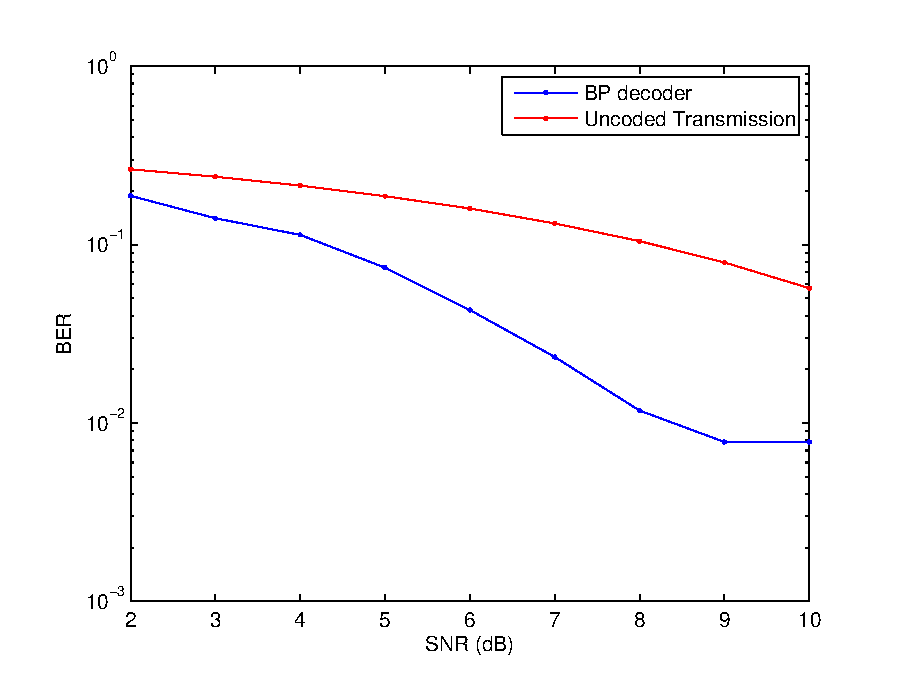
\includegraphics[width=0.8\textwidth]{images/bp}
\caption{BER-SNR curve for the Example LDPC code}
\label{bp}
\end{figure}

\vspace{-2.0em}
\begin{thebibliography}{155}
\bibitem{A}
Shaikh Faisal Zaheer, LDPC Code Simulation (Used for the 128x256 parity check matrix)- 
\\
http://www.mathworks.com/matlabcentral/fileexchange/8977-ldpc-code-simulation. 
\bibitem{AWGN}
AWGN Generation in MATLAB (\textit{addAWGN.m})- \\
http://stackoverflow.com/questions/23690766/proper-way-to-add-noise-to-signal
\end{thebibliography}

\end{document}

